\documentclass{llncs}
%\documentclass[openany,12pt,a4page]{memoir}
%
% Packages
%

\usepackage[utf8]{inputenc}
%\linespread{1.25}\usepackage{listings}
\usepackage{mathptmx}
\usepackage{listings}
\usepackage{xcolor}
\lstdefinestyle{sharpc}{language=[Sharp]C, frame=lr, rulecolor=\color{blue!80!black}}

\definecolor{shcomment}{rgb}{0.12, 0.38, 0.18 } %adjusted, in Eclipse: {0.25, 0.42, 0.30 } = #3F6A4D
\definecolor{shkeyword}{rgb}{0.37, 0.08, 0.25}  % #5F1441
\definecolor{shstring}{rgb}{0.06, 0.10, 0.98} % #101AF9
 \lstset{ % http://stackoverflow.com/questions/741985/latex-source-code-listing-like-in-professional-books
%         basicstyle=\footnotesize\ttfamily,% the size of the fonts
                                % that are used for the code
        basicstyle=\footnotesize\ttfamily,% the size of the fonts that are used for the code
         numbers=left,                     % where to put the line-numbers
         numberstyle=\tiny,                % the size of the fonts that are used for the line-numbers
         stepnumber=1,                     % line numbering steps
         numbersep=5pt,                    % how far the line-numbers are from the code
         tabsize=2,                        % sets default tabsize to 2 spaces
         breaklines=true,                  % sets automatic line breaking
         keywordstyle=\color{shkeyword},        % language function text color
    		frame=b,
 %        keywordstyle=[1]\textbf,    % Stil der Keywords
 %        keywordstyle=[2]\textbf,    %
 %        keywordstyle=[3]\textbf,    %
 %        keywordstyle=[4]\textbf,   \sqrt{\sqrt{}} %
         stringstyle=\color{shstring}, % string text color
%         stringstyle=\color{red},
        commentstyle=\color{shcomment},
         showspaces=false,           % show spaces adding particular underscores
         showtabs=false,             % show tabs within strings adding particular underscores   
         showstringspaces=false,     % underline spaces within strings
         xleftmargin=17pt,
         framexleftmargin=17pt,
         framexrightmargin=5pt,
         framexbottommargin=4pt,
         language=C
 }
\usepackage{caption}
\lstdefinelanguage{Harlan}
{morekeywords={,define,kernel,println,iota,let,main,module,}
sensitive=false,
morecomment=[l]{;},
morecomment=[s]{/*}{*/},
morestring=[b]",
}

\lstdefinelanguage{FSharp}
{morekeywords={,let,float,main,entrypoint,for,parallel,fun,array,printfn,brahma,member,this,module,in,if,else,do,float,try,with,ex,failwith,}
sensitive=false,
morecomment=[l]{//},
morecomment=[s]{(*}{*)},
morestring=[b]",}

\usepackage{tikz}
\usepackage{pgfplotstable}
\usepackage{pgfplots}

%\usepackage{subcaption}
\DeclareCaptionFont{white}{\color{white}}
\DeclareCaptionFormat{listing}{\colorbox[cmyk]{0.43, 0.35, 0.35,0.01}{\parbox{\textwidth}{\hspace{15pt}#1#2#3}}}
\captionsetup[lstlisting]{format=listing,labelfont=white,textfont=white, singlelinecheck=false, margin=0pt, font={bf,footnotesize}}

%% NEW ABOVE Paper Standard Below
\usepackage{enumerate}
\usepackage{amsfonts}
\usepackage{amssymb}
\usepackage{amsmath}
\usepackage{float}
\usepackage[T1]{fontenc}
\RequirePackage[T1]{fontenc}
\RequirePackage{tikz} 
\usepackage{tikz}
\usepackage{amstext}
\usepackage[lofdepth]{subfig}
\usepackage{tabularx}
\usepackage{array}
\usepackage{hyperref}
%\usepackage{url}
\newcolumntype{L}[1]{>{\raggedright\let\newline\\\arraybackslash\hspace{0pt}}m{#1}}
\newcolumntype{C}[1]{>{\centering\let\newline\\\arraybackslash\hspace{0pt}}m{#1}}
\newcolumntype{R}[1]{>{\raggedleft\let\newline\\\arraybackslash\hspace{0pt}}m{#1}}
\usepackage[section]{placeins}
\usepackage[export]{adjustbox}% http://ctan.org/pkg/adjustbox
%\input{macros.tex}

\pagestyle{plain}
\usepackage{array}
\usepackage{wrapfig}
\usepackage{lscape}
\usepackage{rotating}
\usepackage{epstopdf}
%\pgfplotsset{compat=1.5}
\begin{document}

\thispagestyle{empty}
\begin{nopagebreak}
{\samepage 
\begin{tabular}{r}
\parbox{\textwidth}{  \raisebox{11mm}{
\includegraphics[height=1.2cm]{Content/Graphic/aau-logo.jpg}}
\hfill \parbox{4.9cm}{\begin{tabular}{l}
\end{tabular}}}
\\
\end{tabular}

\begin{tabular}{cc}
\parbox{7cm}{
\begin{description}

\item {\textbf Title:} 

CUDAfy og Corecalc 
  
%\item {\textbf Topic:} 
\end{description}

\parbox{8cm}{

\begin{description}
\item {\textbf Project period:}\\
   P10, forår 2016\\
  \hspace{4cm}
\item {\textbf Project Group:}\\
 \href{mailto:nped11@student.aau.dk}{nped11@student.aau.dk}\\
  \hspace{4cm}
\item {\textbf Author:}\\
Niels Br\o ndum Pedersen
  \hspace{2cm}
\item {\textbf Supervisor:}\\
Bent Thomsen
\end{description}
}
\begin{description}
\item {\textbf Total Pages:} - 24
\item {\textbf Completion date:} - 00-00-0000
\end{description}
\vspace\fill} 
\parbox{7cm}{

  \vspace{.15cm}
  \hfill 
  \begin{tabular}{l}
  {\textbf Synopsis:}\bigskip \\
  \fbox{
    \parbox{6.5cm}{\bigskip
     {\vfill{\small In this project, We report on research on making it easier for using a GPU, by using a spreadsheet program as a medium for coding to it. Before the coding of this functionality for a program. a test with matrix multiplication have conducted to see what GPU library best could work in the scope of this project.
The libraries that have been testes are: CUDA, C++ AMP and CUDAfy. it was chosen to make a GPU function using CUDAfy, since it showed promise in the tests and also the open source spreadsheet program that was used, \textit{Corecalc and Funcalc} was made in c\# and CUDAfy was design to be used in that programming language.
There have been conducted a test to see if this new GPU function showed that it coud be useful time wise and these tests showed if the expression that is being calculated is large enough.
     \bigskip}}
     }}
   \end{tabular}}
\end{tabular}}
\\ \\
\noindent{\footnotesize\emph{The content of the report is free to use, yet a official publication (with source references) may only be made by agreement from the authors of the report.}}
\end{nopagebreak}



\newpage

\title{regneark med GPU}

\author{Niels Br\o ndum Pedersen\\ Supervisor: Bent Thomsen}
\institute{Aalborg University, Selma Lagerl\"{o}fsvej 300, DK-9220 Aalborg \O. \\ nped11@student.aau.dk }
%\maketitle
%insert underskrift her med \newpage
\newpage
\section{Intro}
I tidligere Projekt blev der kigget på, om GPU'ens regnekraft kunne bruges i flere programmer for at øge ydeevne. I dette projekt var det også fundet, at det ikke var nemt at programmer til en GPU, fordi metoderne til at kode til en GPU ikke har en godt dokumentation og er kompliceret at lave. Derfor vil jeg i dette projekt prøve at at lave en simple programmering metode for at kunne bruge en GPU's regnekraft GPU, uden man skal havde de store viden inden for det. Regneark bliver brugt af mange og er forholdsvis nemt at programmere, derfor kunne det være interessant, at lave en funktion til et regneark program for at udregne med en GPU. Regneark programment jeg der blev brugt i dette projekt er \textit{Funcalc}\textit{Funcalc} der er open source.
Inden jeg går i gang med at lave GPU funktion vil jeg kigge på tre API for at programmere til en GPU (CUDA, CUDAfy og C++ AMP), for at se hvad der virker godt i forhold til matrix Multiplatikon for at give et godt overblik over hvad der skal bruges når udvidelsen til regnearket skal laves.

Andre har også prøvet at lave det nemmere at kode til en GPU (nogen ref her og eksempler). Det største problem jeg fandt mens jeg arbejde på projektet, var, at igennem CUDA, CUDAfy og C++ AMP ikke gav mulighed for at sende en funktion til GPU, jeg kunne heller ikke finde en smart måde at compile GPU kode på run time, og at når man koder i Excel, bliver det gjort på runtime af programmet der køre excel dokumentet. Måden jeg løste dette problem var ved at sende en opskrift der blev levet efter et abstrakt syntaks træ sammen med data der skal arbejdes på. Med den information vil funktion vide hvordan den skal udregne på den sendte data, dette giver mulighed for at "kode" til en GPU på run time uden at der skal compiles noget på run time. Et anden problem, dog mindre, var at jeg ikke kunne finde løsning på hvordan et program kunne håndtere at bruge forskellige tråde mængder på run time, dette problem jeg jeg kun løst på en meget simple måde der også kan klare forskellige GPU korts.
\section{Relateret Arbejde}
\label{relateret_arbejde}
Det tidligere projekt \cite{P9} blev der kigget på hvad forskellen mellem CPU og GPU, de forskellige metoder til at kode til en GPU. Metoden der blev brugt til at teste det med, var ved at fremstille den samme funktion som et \textit{benchmark} i de forskelle metoder at udregne på, Funktion der blev brugt var \textit{k-means clustering}. Resultatet blev at der er mange måder at programmerer til en GPU, men for at få noget ud af det, skal men havde erfaring og viden ingen for dette område. I projektet blev der kigget på \textit{CUDA}, \textit{AMP}, \textit{F\# Brahma}, \textit{OpenCL} og \textit{Harlan}. 

Artiklen \textit{THE GPU COMPUTING ERA}\cite{nickolls2010gpu} giver et indblik over hvordan \textit{NVIDIA} GPU'er har udviklers sig, samt hvordan man kan kode til dem gennem årende.

Artiklen \textit{A Survey of CPU-GPU Heterogeneous Computing Techniques}\cite{mittalsurvey} beskriver, hvad der er forgået inden for \textit{Heterogene Computing} Teknikker i den videnskabelige ramme. Noget af det der er omtalt er partitonering af arbejdsbyrde for at udnytte CPU'er og GPU'er til at forbedre ydeevnen og/eller energieffektivitet. Der bliver også beskrevet \textit{benchmark} der kan bruges til at evaluere Heterogene computersystemer.

For at gøre noget ved den dårlige beskrivelse af sprogene, der er ved GPU programmering har artiklen \textit{GPU Concurrency: Weak Behaviours and Programming Assumptions}\cite{alglave2015gpu} undersøgt dem. Disse beskrivelsers af sprogene føre til at mange programmører bliver nød til at bruge antagelser ved programmering af software, hvor der gøres brug af GPU. Har denne artikel gennemført en undersøgelse af flere GPU, ved at bruge \textit{litmus} tests. Beskrivelser i programmerings guider og de garantier som leverandørens dokumentation om hardware giver, vil blive undersøgt i omtalte artikel.

Det er ikke kun et problem at kode til en GPU, man skal også kunne vide hvordan information skal gemmes for at få det meste ud af en GPU, som bliver beskrevet i artiklen Artiklen \textit{Adaptive Input-aware Compilation for Graphics Engines}\cite{samadi2012adaptive}.

Til at hjælpe med at fremstille resultater der kunne bruges igennem test af udregnings tid, er Papiret \textit{Microbenchmarks in Java and C\#}\cite{Microbenchmarks} blevet brugt til at hjælpe med at fremstille test programmer, der kunne give resultater angående den brugte tid på at løbe en funktion igennem.

Bogen \textit{Spreadsheet Implementation Technology: Basics and Extensions}\cite{Spreadsheet_Implementation_Technology} er en samling af information inden for programmering af regneark, for at hjælpe programmører der skal i gang med at udvikle til regne ark.

Web bloggen \textit{Collaboration and Open Source at AMD: LibreOffice} \cite{AMD_LibreOffice} beskriver et sammenarbejde mellem dem der har lavet \textit{LibreOffice} og firmaet \textit{AMD}, hvor formålet var at tillade at overføre udregninger i regneark programmet \textit{LibreOffice} til GPU ved at bruge OpenCL. Denne kode blev fremstillet af \textit{AMP} ansatte.

\textit{Spreadsheet optimisation on GPUs} \cite{GPUP2010} er et bachelor projekt som kigger på om det er muligt at bruge GPU til at udregne parallelt i et regnearks program. Programmet som der vil blive udvide på i dette projekt er også \textit{CoreCalc}.

Som dette projekt har planer om at prøve at fuldføre. Her har de brugt \textit{LibreOffice} som regneark programmet til udvikle på og der bliver brugt \textit{OpenCL} for programmering af GPU.
\section{Matrix Multiplatikon}
\label{MM}
For at give et bedre indblik på hvor meget \textit{speed-up} det giver at bruge GPU'en i forhold til CPU'en, er der fremstillet simpel programmer der går en matrix multikapion igennem. Der er lavet to versioner for hver GPU biblioteker, der er blevet kigget på. Forskellen mellem versionerne er, at den ene gør brug af en dimension og den anden bruger to dimensioner for array. De biblioteker der er blevet tested er \textit{C++ AMP}, \textit{CUDA} og \textit{CUDAfy}.

Testene bliver gjort for at give et bedre indblik på de forskellige valgte metoder til at kode til en GPU, om der er nogen forskel på hvordan input til GPU ser ud i forhold til om speed-up. Derefter er der blevet lavet et test program med \textit{C++ AMP} der bliver kaldt fra C\# kode, for at se hvordan dette kunne gøres og om det har den store effekt på udregnings tid med at bruge denne metode der er blevet fundet. Dette bliver gjort for fordi programmet Funcalc er skrevet i C\#.

Test metoden er blevet fremstillet efter artiklen \textit{Microbenchmarks in Java and C\#} \cite{Microbenchmarks}. Af de versioner af test artiklen beskriver bruges der \textit{Mark4} version.

Koden der bliver gået igennem er \textit{CUDAfy} med en dimension \textit{array}. På figure \ref{fig:MainPart1} kan del et af koden for \textit{Main} funktion ses. \textit{testSize} er de forskellige størrelser der vil blive taget tid på, eksempelvis når den tester med værdien 20, vil den lave 2 matrixer der har størrelsen 20 X 20. Siden koden der bliver vist her, er for en dimension \textit{array}, vil den lave \textit{array} med \textit{Size1d}, der er \textit{Size} ganget med sig selv. værdierne der bliver lavet på linje 3 styrer hvor mange gange \textit{Mark4}, variablen \textit{n} er hvor mange gange der skal tages tid på den samme størrelses og  \textit{count} er hvor mange gange funktion skal gøres mens der tages tid. 

\textit{For} løkken der mellem på linje 5 og 22, bruges til at køre \textit{testSize} og lave en Mark 4 test med matrixer med størrelsen beskrevet i \textit{testSize}. Fra linje 7 til 16 vil de to \textit{array} simpel blive lavet, disse \textit{array} bruges til input for matrix multiplatikon. På linje 18 vil \textit{Mark4} blive kaldt, den vil returner to tal empirisk middelværdi og standard
afvigelsen, der vil blive lagt ned i et \textit{array} \textit{result}, der kommer til at holde resultaterne fra alle testende for dette program, samt størrelsen der blev testet.

\begin{figure}[h]
    \centering
    \lstset{style=sharpc}
	\begin{lstlisting}
int[] testSize = new int[] { 5, 10, 20, 50, 100, 200, 300, 400, 500, 600, 700, 800, 900, 1000 };
            double[,] result = new double[testSize.Length, 3];
            int i, n = 10, count = 100;
            
            for (i = 0; i < testSize.Length; i++)
            {
                int Size = testSize[i];
                int Size1d = Size * Size;
                int[] A = new int[Size1d];
                int[] B = new int[Size1d];
                int[] C = new int[Size1d];
                for (int x = 0; x < (Size1d); x++)
                {
                    A[x] = 2;
                    B[x] = 3;
                }
                Console.WriteLine(testSize[i] + " starting");
                double[] Mark4_time = Mark4(A, B, C, Size, Size1d, n, count);
                result[i, 0] = testSize[i];
                result[i, 1] = Mark4_time[0];
                result[i, 2] = Mark4_time[1];
            }
	\end{lstlisting}
    \caption{Første del af \textit{Main} for CUDAfy matrix multiplatikon med en dimension \textit{array}.}
    \label{fig:MainPart1}
\end{figure}

Det næste til der vil blive beskrevet er \textit{Mark4} som kan ses på figure \ref{fig:Mark4}. Fra linje 6 til 12 bliver GPU information fundet og gemt, samt fundet ud hvor mange tråde der max kan være i en block. Denne information bliver lavet inden målingen starter, siden denne information kan laves starten af programmet og blive genbrugt. Fra linje 14 til linje 23 er hovede delen i \textit{Mark4}, her vil \textit{MA}, forkortelse for \textit{matrix multiplikation Algoritme}, blive testet igennem og taget tid på ved at bruge \textit{timer} klassen der kan ses påkode snippet\ref{fig:timer}.

\begin{figure}[h]
    \centering
    \lstset{style=sharpc}
	\begin{lstlisting}
public static double[] Mark4(int[] A, int[] B, int[] C, int Size, int Size1d, int n, int count)
        {
            double dummy = 0.0;
            double st = 0.0, sst = 0.0;

            CudafyModule km = CudafyTranslator.Cudafy();

            GPGPU gpu = CudafyHost.GetDevice(CudafyModes.Target, CudafyModes.DeviceId);
            gpu.LoadModule(km);

            GPGPUProperties GPU_prop = gpu.GetDeviceProperties();
            int max_threadsPerBlock = GPU_prop.MaxThreadsPerBlock;

            for (int j = 0; j < n; j++)
            {
                Timer t = new Timer();
                for (int i = 0; i < count; i++)
                    dummy += MA(A, B, C, Size, Size1d, gpu, max_threadsPerBlock);
                double time = t.Check() / count;
                st += time;
                sst += time * time;
            }
            double mean = st / n, sdev = Math.Sqrt((sst - mean * mean * n) / (n - 1));
            return new double[2] { mean, sdev };
        }
	\end{lstlisting}
    \caption{\textit{Mark4} klassen der bliver brugt til at teste med.}
    \label{fig:Mark4}
\end{figure}

\begin{figure}[h]
    \centering
    \lstset{style=sharpc}
	\begin{lstlisting}
// timer class taken from the paper: Microbenchmarks in Java and C# by Peter Sestoft (sestoft@itu.dk) IT University of Copenhagen, Denmark
    // plan on using Mark4 for tests
    class Timer
    {
        private readonly System.Diagnostics.Stopwatch stopwatch = new System.Diagnostics.Stopwatch();
        public Timer() { Play(); }
        public double Check() { return stopwatch.ElapsedMilliseconds; }
        public void Pause() { stopwatch.Stop(); }
        public void Play() { stopwatch.Start(); }
    }
	\end{lstlisting}
    \caption{Timer klassen taget fra artiklen \textit{Microbenchmarks in Java and C\#} \cite{Microbenchmarks}.}
    \label{fig:timer}
\end{figure}

Funktion \textit{MA} kan ses på figure \ref{fig:MA}. på linjerne 4 til 6 kan det ses at der bliver allokeret plads på GPU, på linje 9 og 10 bliver data flyttet over på GPU, fra linje 12 til 24 vil den finde ud af hvor tråde og blokke der skal bruges for at kunne gennemgå funktions input. På linje 27 vil GPU funktion blive kørt, hvorefter på linje 30 vil man flytte resultatet fra GPU tilbage til CPU og til sidst vil \textit{array} der er blevet allokeret blive frigivet.

\begin{figure}[h]
    \centering
    \lstset{style=sharpc}
	\begin{lstlisting}
public static int MA(int[] A, int[] B, int[] C, int Size, int Size1d, GPGPU gpu, int max_threadsPerBlock)
        {
            // allocate the memory on the GPU
            int[] GPU_A = gpu.Allocate<int>(A);
            int[] GPU_B = gpu.Allocate<int>(B);
            int[] GPU_C = gpu.Allocate<int>(C);

            // copy the arrays 'a' and 'b' to the GPU
            gpu.CopyToDevice(A, GPU_A);
            gpu.CopyToDevice(B, GPU_B);

            int threadsPerBlock = 0;
            int blocksPerGrid = 0;

            if (Size1d < max_threadsPerBlock)
            {
                threadsPerBlock = Size1d;
                blocksPerGrid = 1;
            }
            else
            {
                threadsPerBlock = max_threadsPerBlock;
                blocksPerGrid = (Size1d / max_threadsPerBlock) + 1;
            }

            // launch GPU_MA
            gpu.Launch(threadsPerBlock, blocksPerGrid).GPU_MA(GPU_A, GPU_B, GPU_C, Size, Size1d);

            // copy the array 'c' back from the GPU to the CPU
            gpu.CopyFromDevice(GPU_C, C);

            gpu.Free(GPU_A);
            gpu.Free(GPU_B);
            gpu.Free(GPU_C);
            return 1;
        }
	\end{lstlisting}
    \caption{\textit{matrix multiplikation Algoritme} funktion.}
    \label{fig:MA}
\end{figure}

På kode snittet \ref{fig:GPU_MA} kan koden der bruges på GPU ses. Måden at en tråd finder dens ide på, er ved at gøre brug af \textit{thread.threadIdx}. Men dette er ikke nok fordi \textit{thread.threadIdx} giver dens id i den block den nu befinder sig i, Derfor skal der også bruges \textit{thread.blockIdx} der giver id på den block tråden befinder sig i.

\begin{figure}[h]
    \centering
    \lstset{style=sharpc}
	\begin{lstlisting}
[Cudafy]
        public static void GPU_MA(GThread thread, int[] GPU_A, int[] GPU_B, int[] GPU_C, int Size, int Size1d)
        {
            int i = thread.threadIdx.x + thread.blockDim.x * thread.blockIdx.x;

            if (i < Size1d)
            {
                GPU_C[i] = 0;
                int x = i / Size;
                int y = i % Size;
                for (int z = 0; z < Size; z++)
                {
                    GPU_C[i] += GPU_A[(x * Size) + z] * GPU_B[(z * Size) + y];
                }
            }
        }
	\end{lstlisting}
    \caption{GPU funktion til \textit{matrix multiplikation Algoritme}.}
    \label{fig:GPU_MA}
\end{figure}

For at gøre det mere overskueligt at kigge på resultaterne vil \textit{Main} part 2 lave en tekst fil med resultaterne i og gemme filen, kode snippet \ref{fig:MainPart2} viser denne del.


\begin{figure}[h]
    \centering
    \lstset{style=sharpc}
	\begin{lstlisting}
string lines = "CUDAfy 1D MA in C Sharp  mean  , sdev \r\n";
            for (i = 0; i < testSize.Length; i++)
            {
                lines = lines + "size: " + result[i, 0] + " time: " + result[i, 1] + " " + result[i, 2] + "\r\n";
            }

            // Write the string to a file.
            string path = @"c:\result\CUDAfy_1D_MA_in_C_Sharp.txt";
            System.IO.StreamWriter file;
            if (!System.IO.File.Exists(path))
            {
                file = System.IO.File.CreateText(path);

            }
            else
            {
                file = new System.IO.StreamWriter(path);
            }
            file.WriteLine(lines);
            file.Close();
	\end{lstlisting}
    \caption{Anden del af \textit{Main} for \textit{CUDAfy} matrix multiplatikon med en dimension \textit{array}.}
    \label{fig:MainPart2}
\end{figure}
































\section{Test af Matrix Multiplatikon}
I denne det vil resultaterne af testende på en computer med udstyret blive vist:
\begin{itemize}
\item styresystem: Windows 10 Pro N
\item Processor: intel core i5-4690K
\item Hukommelse (RAM): 12 GB
\item Skærmkort: NVIDIA GeForce GTX 960
\end{itemize}

\subsection{Resultater fra Programmerne} \label{result_GPU_Funcalc}
resultater vil blive delt op efter hvad tiden er blevet målt igennem, C\# og C++. Dette er gjort fordi at C\# har muligheden for at måle i tid, kan man ikke rigtig måle i tid i C++. I C++ kan man bruge biblioteket \textit{time.h}, problemet med dette biblioteket er, at det måler i \textit{clock ticks}, der er en tidsenhed af en konstant, men systemspecifikke længde. Der findes en macro \textit{CLOCKS\_ PER\_ SEC}, som burde gøre arbejde, men med mine test kan kan jeg ikke se hvordan det passer sammen med hvad jeg får med mine C\# målinger.

På tabel \ref{fig:samletCS} kan målingerne fra C\# ses og på tabel \ref{fig:samletC++} kan målingerne fra C++ ses. C++ AMP med to dimensioner array skete der en stack overflow da array blev på størrelse 300 x 300 eller over.

% ------------------------------------------------------------------------------------------------------------- samlet C#
\begin{figure}[p]
    \centering
   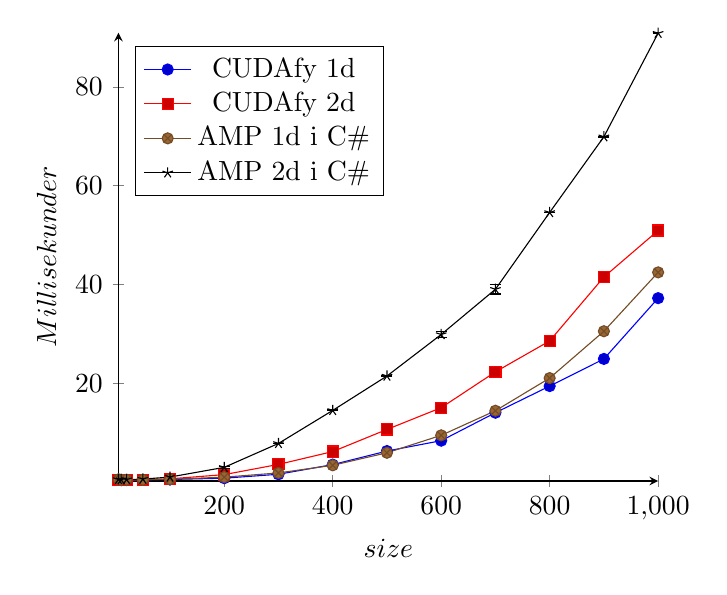
\begin{tikzpicture} 
\begin{axis}
[
    axis lines = left,
    xlabel = $size$,
    ylabel = $Millisekunder$,
    legend pos=north west,
]

 \addplot+[error bars/.cd,y dir=both,y explicit]
	coordinates 
    	{ 	
		(5,0.533) +- (0,0.147)
		(10,0.478) +- (0,0.019)
		(20,0.487) +- (0, 0.010)
		(50,0.543) +- (0,0.012)
		(100,0.607) +- (0,0.012)
		(200,0.87) +- (0,0.013)
		(300, 1.661) +- (0,0.041)
		(400,3.617) +- (0,0.047)
		(500,6.359) +- (0,0.107)
		(600,8.456) +- (0,0.096)
		(700,14.109) +- (0,0.050)
		(800,19.492) +- (0,0.035)
		(900,24.987) +- (0, 0.036)
		(1000,37.275) +- (0,0.029)
 }; \addlegendentry{CUDAfy 1d}
 \addplot+[error bars/.cd,y dir=both,y explicit]
	coordinates 
    	{ 	
		(5,0.499) +- (0,0.033)
		(10,0.492) +- (0,0.010)
		(20,0.499) +- (0, 0.005)
		(50,0.56) +- (0,0.014)
		(100,0.74) +- (0,0.014)
		(200,1.594) +- (0,0.013)
		(300,3.658) +- (0,0.116)
		(400,6.251) +- (0,0.213)
		(500,10.728) +- (0,0.062)
		(600,15.122) +- (0,0.049)
		(700,22.367) +- (0,0.051)
		(800,28.626) +- (0,0.039)
		(900,41.546) +- (0, 0.025)
		(1000,50.958) +- (0,0.011)
 }; \addlegendentry{CUDAfy 2d}
 
\addplot+[error bars/.cd,y dir=both,y explicit]
	coordinates 
    	{ 	
		(5,0.637) +- (0,0.342)
		(10,0.556) +- (0,0.022)
		(20,0.56) +- (0, 0.0205)
		(50,0.552) +- (0,0.011)
		(100,0.656) +- (0,0.026)
		(200,1.076) +- (0,0.032)
		(300, 1.931) +- (0,0.046)
		(400,3.478) +- (0,0.017)
		(500,6.009) +- (0,0.018)
		(600,9.534) +- (0,0.021)
		(700,14.509) +- (0,0.023)
		(800,21.107) +- (0,0.014)
		(900,30.587) +- (0, 0.020)
		(1000,42.488) +- (0,0.039)
 };  \addlegendentry{ AMP 1d i C\#}
 
 \addplot+[error bars/.cd,y dir=both,y explicit]
	coordinates 
    	{ 	
		(5,0.611) +- (0,0.180)
		(10,0.562) +- (0,0.014)
		(20,0.581) +- (0, 0.012)
		(50,0.685) +- (0,0.007)
		(100,1.099) +- (0,0.008)
		(200,3.061) +- (0,0.232)
		(300, 7.895) +- (0,0.027)
		(400,14.574) +- (0,0.080)
		(500,21.529) +- (0,0.182)
		(600,29.924) +- (0,0.685)
		(700,39.074) +- (0,0.964)
		(800,54.605) +- (0,0.070)
		(900,69.917) +- (0, 0.117)
		(1000,90.851) +- (0,0.098)
 }; \addlegendentry{ AMP 2d i C\#}
\end{axis} \end{tikzpicture}    
    \caption{ alle målinger der er lavet i C\#}
    \label{fig:samletCS}
\end{figure}

% ------------------------------------------------------------------------------------------------------------- samlet C++
\begin{figure}[p]
    \centering
   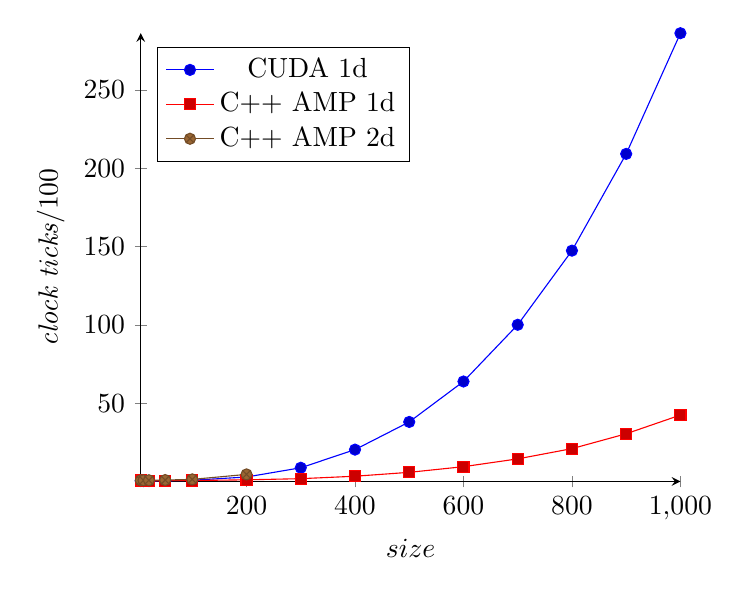
\begin{tikzpicture} 
\begin{axis}
[
    axis lines = left,
    xlabel = $size$,
    ylabel = $\textit{clock ticks}/100$,
    legend pos=north west,
]
\addplot+[error bars/.cd,y dir=both,y explicit]
	coordinates 
    	{ 	
		(5,0.542) +- (0,0.242)
		(10,0.477) +- (0,0.014)
		(20,0.498) +- (0, 0.007)
		(50,0.609) +- (0,0.008)
		(100,0.984) +- (0,0.021)
		(200,3.063) +- (0,0.035)
		(300, 8.957) +- (0,0.114)
		(400,20.526) +- (0,0.106)
		(500,38.194) +- (0,0.027)
		(600,63.997) +- (0,0.027)
		(700,100.162) +- (0,0.020)
		(800,147.458) +- (0,0.135)
		(900,209.182) +- (0, 0.025)
		(1000,286.169) +- (0,0.046)
 }; \addlegendentry{ CUDA 1d}
 
 \addplot+[error bars/.cd,y dir=both,y explicit]
	coordinates 
    	{ 	
		(5,0.826) +- (0,0.373)
		(10,0.7) +- (0,0.020)
		(20,0.694) +- (0, 0.013)
		(50,0.714) +- (0,0.034)
		(100,0.819) +- (0,0.017)
		(200,1.266) +- (0,0.021)
		(300, 1.999) +- (0,0.07)
		(400,3.56) +- (0,0.038)
		(500,6.042) +- (0,0.039)
		(600,9.649) +- (0,0.016)
		(700,14.629) +- (0,0.017)
		(800,21.16) +- (0,0.012)
		(900,30.643) +- (0, 0.027)
		(1000,42.58) +- (0,0.044)
 }; \addlegendentry{ C++ AMP 1d}
 
 \addplot+[error bars/.cd,y dir=both,y explicit]
	coordinates 
    	{ 	
		(5,0.945) +- (0,0.677)
		(10,0.948) +- (0,0.637)
		(20,0.995) +- (0, 0.769)
		(50,1.122) +- (0,0.798)
		(100,1.550) +- (0,0.771)
		(200,4.725) +- (0,0.588)
 }; \addlegendentry{ C++ AMP 2d}

\end{axis} \end{tikzpicture}    
    \caption{samlet C++}
    \label{fig:samletC++}
\end{figure}

\subsection{resultat af testen}
Ud fra testen virker det som om at CUDAfy er et godt valg til at kode i, når det skal gøres i C\# . Derfor vil GPU funktion der laves i dette projekt bruge CUDAfy til at lave GPU delen med.





\section{GPU Funktion}
\label{GPU_F}
I dette projekt havde jeg planer om, at lave en ekstra funktion til \textit{CoreCalc} for at kunne "kode" til GPU igennem regnearket. Funktion har jeg kaldt \emph{GPU}, man skal markere de felter man vil bruge som output, ligesom funktion \textit{TRANSPOSE}. \emph{GPU} har 2 input, det første er et \textit{array}, eller et data sæt, der marker det data der skal udregnes på, og det andet er et \textit{CoreCalc} udtryk/funktion, hvor talende i udtrykket peger til hvilken kolonne i den data den skal indsætte på dette placering i udregningen.

På figure \ref{fig:corecalc1} kan der ses et billede af \textit{CoreCalc} hvor \textit{GPU} er i brug. A1 til B6 er data sættet der vil blive brugt som input til \textit{GPU}. I C6 kan \textit{GPU} funktion beskrivelsen blive set, den tager A1 til B6 som input \textit{array} (A1:B6) og et udtryk (1+2), som beskriver til \textit{GPU} at kolonne 1 skal plusset(+) samme med kolonne 2. Bemærk at C1 til C6 er markeret mens at funktion bliver skrevet, dette bliver gjort fordi at \textit{GPU} output også er at \textit{array}, så derved viser du \textit{GPU} funktion hvor dens output skal være. Bemærk også det markeret område har lige så mange rækker som input har.

For at lave GPU funktion, vil klassen \textit{Function} i \textit{Corecalc and Funcalc} blive modificeret for at kunne kalde GPU funktion. I figure \ref{fig:corecalc_class} kan et klasse diagram ses over klasserne i \textit{Corecalc and Funcalc}. pilen der er peger på \textit{Function} klassen.

\begin{figure}[p]
    \centering
    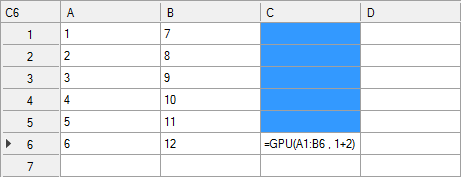
\includegraphics[width=0.8\textwidth]{Content/Graphic/corecalc1.png}
    \caption{et billede af \textit{CoreCalc} hvor \textit{GPU} bliver brugt.}
    \label{fig:corecalc1}
\end{figure}

\begin{figure}[p]
    \centering
    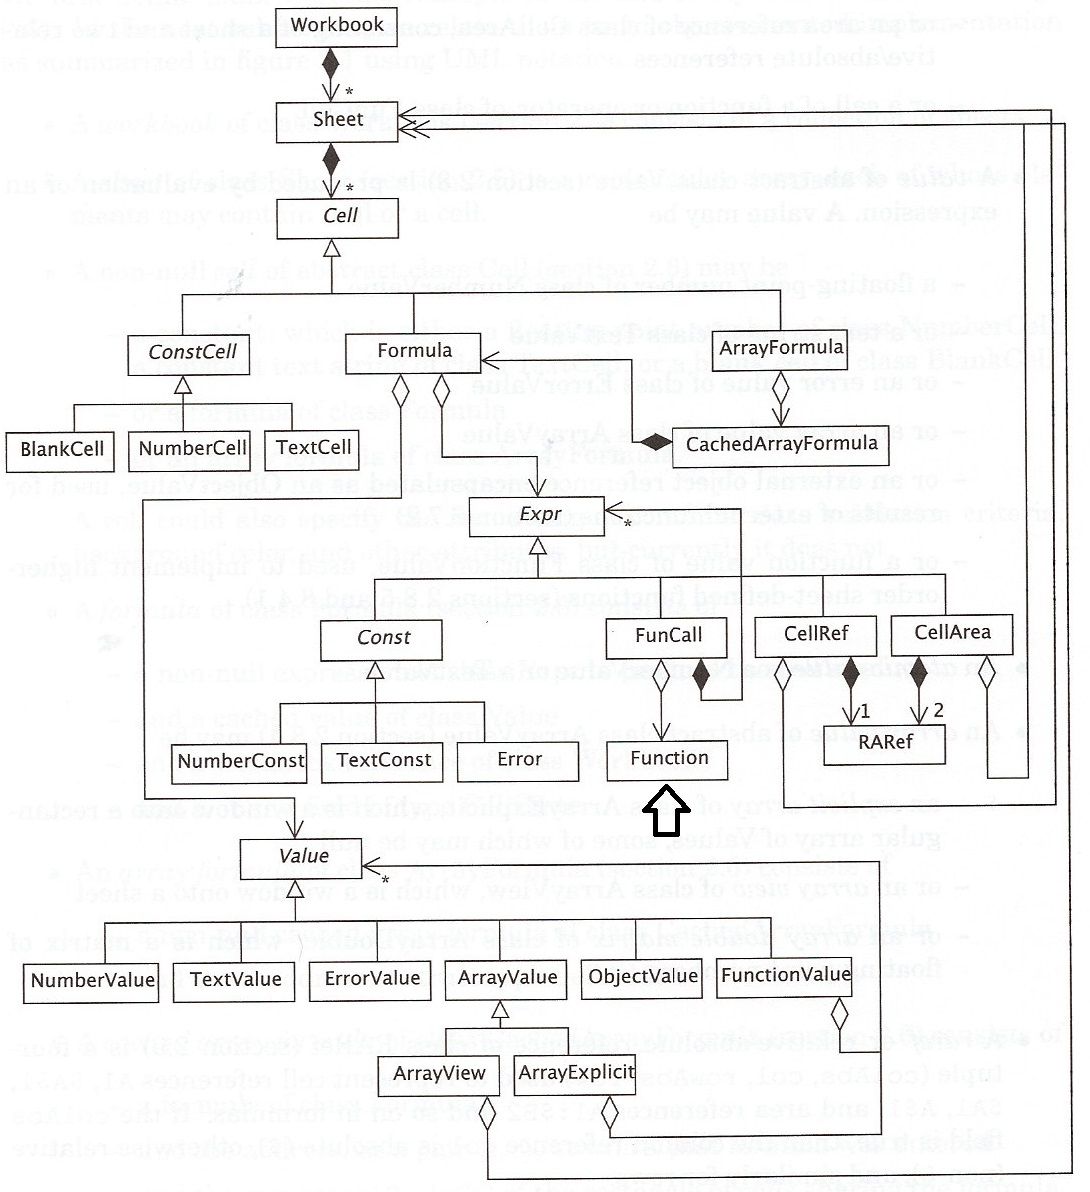
\includegraphics[width=0.8\textwidth]{Content/Graphic/CorecalcClass.png}
    \caption{Grafs over klasserne i \textit{Corecalc and Funcalc}, taget fra bogen \textit{Spreadsheet optimisation on GPUs} \cite{GPUP} side 30. pilen peger på klassen der vil blive lavet i, for at kunne bruge GPU funktion.}
    \label{fig:corecalc_class}
\end{figure}
\section{GPU-calculate til CoreCalc}
\label{GPU_CC}
I dette projekt vil CUDAfy blive brugt, til at øge regnekræften i open source programmet \textit{Funcalc} der kan findes på hjemmesiden \cite{FuncalcHome}.
\textit{Funcalc} en udvidelse til \textit{Corecalc}, der er en implementering af et regneark funktionalitet lavet i sproget C\#, det er lavet som et forskning prototype som ikke er lavet til at kunne blive brugt i stedet for de officielse versioner, såsom Microsoft Excel.

Klassen \textit{GPU\_ func} i \textit{GPU\_ calculate} mappen er hvor det meste arbejde ligger fra dette projekt. For at kunne bruge det, har jeg også tilført noget kode i klassen \textit{Function} i \textit{Corecalc}.

\subsection{GPU\_ func}
Klassen \textit{GPU\_ func} er der seks funktioner og en konstruktør.

Konstruktøren bliver brugt til at hente information om GPU'en, der bruges til at bestemme om en blok er nok, hvis ikke hvor mange blokke skal der så bruges. Grunden til at information bliver hentet, når man laver klassen er for minimere tiden funktion skal bruge på udregning, da jeg har observeret, at det tager en god potion tid at hente denne information. Konstruktøren og de globale variabler kan ses i figure \ref{fig:GPU_func_K}, \textit{tempResult} bliver brugt i \textit{makeFuncHelper} til at styre hvad for nogen midlertidig variable er i brug.

\begin{figure}[!ht]
    \centering
    \lstset{style=sharpc}
	\begin{lstlisting}
class GPU_func
    {
        private CudafyModule km;
        private GPGPU gpu;
        private GPGPUProperties GPU_prop;
        private List<int> tempResult;
        
        public GPU_func()
        {
            km = CudafyTranslator.Cudafy();

            gpu = CudafyHost.GetDevice(CudafyModes.Target, CudafyModes.DeviceId);
            gpu.LoadModule(km);

            GPU_prop = gpu.GetDeviceProperties();
        }
	\end{lstlisting}
    \caption{konstruktøren for \textit{GPU\_ func} samt de globale værdier der bliver brugt i klassen}
    \label{fig:GPU_func_K}
\end{figure}

\subsection{makeFunc}
\textit{makeFunc} og \textit{makeFuncHelper} funktionerne bruges til at fremstille en indkodning af hvordan hvordan GPU'en skal udregne, ud fra at abstrakt syntaks træ af et udtryk. Denne liste har \textit{X} antal a fire tal som er en enkle udregning (+,-,*,/) med to værdier, \textit{X} er hvor mange udregning er skal gøres i alt, for at komme til resultatet som udtrykket vil give.

Tallene i den enkle udregning har en bestemt mening, første og tredje tal er hvad variabler der skal gøres noget med, det andet tal er for at bestemme hvilken udregning der skal gøres (+,-,*,/) og det fjerde og sidste bliver brugt til at bestemme om resultatet skal lige ligges i en midlertidig variable eller om den skal ligges i resultat listen.

\textit{makeFuncHelper} kan ses i fem dele. Første del kan ses på figure \ref{fig:makeFuncHelper_part_1} hvor den finder ud af om input variabler er en funktion eller en værdi. Det skal pointeres at \textit{makeFuncHelper} er en rekursiv funktion, der er lavet for at gå igennem det abstrakt syntaks træ nemt.

\begin{figure}[!ht]
    \centering
    \lstset{style=sharpc}
	\begin{lstlisting}
private List<List<int>> makeFuncHelper(FunCall input, bool root)
        {
            List<List<int>> temp = new List<List<int>>();
            int locationOne = 0, locationTwo = 0; // used to hold the temp locating of the result
            // find where to place output

            bool oneIsFunc = (input.es[0] is FunCall);
            bool oneIsNumber = (input.es[0] is NumberConst);
            bool twoIsFunc = (input.es[1] is FunCall);
            bool twoIsNumber = (input.es[1] is NumberConst);
	\end{lstlisting}
    \caption{Første del af \textit{makeFuncHelper} som kigger på variabler af input.}
    \label{fig:makeFuncHelper_part_1}
\end{figure}

Anden del kan ses på figure \ref{fig:makeFuncHelper_part_2}, denne del arbejder med inputs variablerne. Fra linje 1 til 13 er for første værdi, hvis denne værdi er en funktion, vil den kalde sig selv med funktion som input, Hvis det er en værdi, vil den tage værdien og ligge den ned i \textit{locationOne}, som er værdien der holder styr på, hvor \textit{GPUFunc} skal tage information fra for hver udregning trin. Det samme sker så for anden inputs variablerne fra linje 14 til 27.

\begin{figure}[!ht]
    \centering
    \lstset{style=sharpc}
	\begin{lstlisting}
            if (oneIsFunc)
            {
                temp.AddRange(makeFuncHelper(input.es[0] as FunCall,false));
                locationOne = temp[temp.Count - 1][3];
            }
            else if(oneIsNumber)
            {
                locationOne = (int)Value.ToDoubleOrNan((input.es[0] as NumberConst).value);
            }
            else
            {
                // some kind of error...
            }
            if (twoIsFunc)
            {
                temp.AddRange(makeFuncHelper(input.es[1] as FunCall, false));
                locationTwo = temp[temp.Count - 1][3];
               
            }
            else if (twoIsNumber)
            {
                locationTwo = (int)Value.ToDoubleOrNan((input.es[1] as NumberConst).value);
            }
            else
            {
                // some kind of error...
            }
	\end{lstlisting}
    \caption{Anden del af \textit{makeFuncHelper} der laver arbejdet med inputs variabler.}
    \label{fig:makeFuncHelper_part_2}
\end{figure}

Den tredje kigger på hvilket form for udregning/operation der bliver gjort i input, dette kan ses i figure \ref{fig:makeFuncHelper_part_3}

\begin{figure}[!ht]
    \centering
    \lstset{style=sharpc}
	\begin{lstlisting}
            int functionValue = 0; ;
            string function = input.function.name.ToString();
            switch (function)
            {
                case "+":
                    functionValue = 1;
                    break;
                case "-":
                    functionValue = 2;
                    break;
                case "*":
                    functionValue = 3;
                    break;
                case "/":
                    functionValue = 4;
                    break;
                default:
                    // some kind of error...
                    break;
            }
	\end{lstlisting}
    \caption{Tredje del af \textit{makeFuncHelper} finder ud af hvad for en operation der sker i input.}
    \label{fig:makeFuncHelper_part_3}
\end{figure}

Fjerde del der kan ses på figure \ref{fig:makeFuncHelper_part_4} stater med at lave en liste \textit{result}, der bliver brugt til holde indkodning af input i dette point i det abstraktet syntaks træ.

Hvis der har været brugt midlertidig variable for dens input variabler, vil den fjerne dem fra listen fra brugte midlertidig variable liste \textit{tempResult}. Dette er gjort for at spare på pladsen på GPU ved at genbruge midlertidig variable placeringer, hvor det er muligt.

\begin{figure}[!ht]
    \centering
    \lstset{style=sharpc}
	\begin{lstlisting}
            List<int> result = new List<int>();

            if (oneIsFunc)
            {
                tempResult.RemoveAt(tempResult.FindLastIndex(x => x == locationOne));
            }
            if(twoIsFunc)
            {
                tempResult.RemoveAt(tempResult.FindLastIndex(x => x == locationTwo));
            }

            int outputPlace = 0;
            if(!root)
            { 
                int x = -1;
                while (outputPlace == 0)
                {
                    if(!tempResult.Contains(x))
                    {
                        outputPlace = x;
                    }
                    else
                    {
                        x--;
                    }
                }
            }
            tempResult.Add(outputPlace);
	\end{lstlisting}
    \caption{Fjerde del af \textit{makeFuncHelper} fjerner brugt midlertidig variabler placeringer for genbrug og finde ud af hvor inputs resultat skal placeres.}
    \label{fig:makeFuncHelper_part_4}
\end{figure}

Den femte og sidste del \ref{fig:makeFuncHelper_part_5} i \textit{makeFuncHelper} gemmer hvad de tidligere dele har fundet ind i listen \textit{result} og returner \textit{temp}  der er en liste af lister, efter at have lagt \textit{result} på den.

\begin{figure}[!ht]
    \centering
    \lstset{style=sharpc}
	\begin{lstlisting}
            result.Add(locationOne);
            result.Add(functionValue);
            result.Add(locationTwo);
            result.Add(outputPlace);

            temp.Add(result);

            return temp;
	\end{lstlisting}
    \caption{Femte del af \textit{makeFuncHelper} sætter alt sammen og sender hvad den har fundet ud af tilbage.}
    \label{fig:makeFuncHelper_part_5}
\end{figure}

For at give et eksempel på hvorden \textit{makeFunc} gør, kan vi tage regnestykket \textit{(1+2)*(3+4)}, det her ses om en kommando for GPU funktion hvor tallene bliver brugt til at bestemme hvilken kolonne, den skal tag værdien fra. Den kunne komme til at se sådan ud: (1,1,2,-1),(3,1,4,-2),(-1,3,-2,0). 1+2 er blevet lavet om til (1,1,2,-1), 3+4 er blevet om til (3,1,4,-2) og ()*() er lavet til (-1,3,-2,0). Grunden til at der står minus -1 og -2 ved udregningen for 1+2 og 3+4, er at minus værdier bliver brugt til at beskrive midlertidig variabler og 0 for output. Eg bliver \textit{(1+2)*(3+4)} til en liste der kan se sådan ud
\begin{itemize}
 \item 1,1,2,-1
 \item 3,1,4,-2
 \item -1,3,-2,0
\end{itemize}


\subsection{findnumberOfTempResult}
Dette er en simple funktion der går gennem en indkodningen og finder det antal af midlertidig resultater der skal bruges i indkodningen.

\subsection{calculate}
Når man skal bruge en GPU gennem CUDA og CUDAfy skal man gøre forskellige ting, disse ting bliver gjort her. Variablerne \textit{numberOfTempResult}, \textit{SizeOfInput},  \textit{AmountOfNumbers} og \textit{numberOfFunctions} bliver lavet til at starte med. \textit{SizeOfInput} er hvor mange koloner der er med i input, \textit{AmountOfNumbers} er hvor mange rækker der med i input.

Der bliver lavet to \textit{array} \textit{output} og \textit{tempResult}. \textit{tempResult} Bliver brugt til holde midlertidig resultater på GPU når indkodning af udtrykket bliver læst igennem, grundet dette bliver gjort her, er at antal af midlertidig resultater der skal gemmes i en funktion kan variere alt efter hvor kompliceret den er og efter hvad der er fundet på nettet, giver CUDAfy ikke mulighed for at lave et \textit{array} på run time på GPU tråde lokale hukommelse.

Det første der bliver udregnet er, hvor mange block og tråde der skal bruges, alt efter hvad hardware kan håndter.

Derefter vil alle \textit{array} få allokeret plads på GPU. De \textit{array} der bliver sent til GPU, vil være dem med information om input data og indkodning af udtrykket, \textit{array} der er blevet allokeret for de midlertidig resultater vil ikke blive send til GPU, da dette \textit{array} ikke holder information fra CPU, som GPU skal bruge.

Hvorefter vil de, der har nødvendig data blive send over. Derefter vil selve GPU funktion blive kaldt. Derefter vil output data blive hente tilbage fra GPU og til sidst vil den hukommelse der er brugt på \textit{array} blive frigivet.

\subsection{GPUFunc}
\textit{GPUFunc} er funktion der vil blive kørt på GPU. Den har tre ting den gør for hver punkt i indkodningen. Først vil den finde de variabler den skal bruge, midlertidig eller fra input, så vil den gøre noget med de to variabler den har fundet, +,-,*,/, og til sidst vil den finde ud af hvor output skal lægges hen. Koden har meget til fælles med \textit{makeFuncHelper}, på grund af den læser indkodningen og udregner alt efter, hvad indkodningen beskriver i sted for at lave en indkodningen.


\subsection{kode i Corecalc Function klasse}
Koden der lavet i \textit{Function} klassen i \textit{Corecalc}, der har bundet GPU koden sammen til resten af \textit{Corecalc}. Der er tre forskellige steder, at kode er blevet sat ind, selve \textit{Function} har fået en private \textit{GPU\_func GPU} der bliver initierets når \textit{Function} bliver. For at GPU funktion skal kunne blive kaldt, er den blevet sat ind i tabellen af funktioner. De linjer der er sat ind kan ses  på figure  \ref{fig:Corecalc_FC_1}.

\begin{figure}[!ht]
    \centering
    \lstset{style=sharpc}
	\begin{lstlisting}
              GPU = new GPU_func();
              .
              .
              .
              new Function("GPU", GPUFunction()); //GPUFUNC
	\end{lstlisting}
    \caption{Ting der er lavet i \textit{Function} konstruktøren.}
    \label{fig:Corecalc_FC_1}
\end{figure}


Den sidste del af koden i denne klasse ligger i \textit{GPUFunction}, kan ses i figure \ref{fig:Corecalc_FC_2}, koden her er samlelede mellem \textit{Corecalc} og \textit{GPU\_ func}. Kodens opgave er tage funktions kaldet input og lave det til information som \textit{GPU\_ func} klassen vil kunne bruge til at udregne med, det gør den ved at hente det beskrevet \textit{array}, lave det om til et double \textit{array}, derefter tager den det andet input og laver om til en indkodning. Med indkodningen og double \textit{array} kan den kalde \textit{calculate} der giver et double \textit{array} tilbage med resultaterne, til sidst vil den fremstille et \textit{Corecalc} \textit{value} \textit{array}, hvor resultatet vil blive kopieret over i og derefter vil blive sent tilbage.

\begin{figure}[!ht]
    \centering
    \lstset{style=sharpc}
	\begin{lstlisting}
    private static Applier GPUFunction()
    {
        return
          delegate(Sheet sheet, Expr[] es, int col, int row)
          {
              if (es.Length == 2)
              {
                  Value v0 = es[0].Eval(sheet, col, row);
                  
                  if (v0 is ErrorValue) return v0;
                  ArrayValue v0arr = v0 as ArrayValue;
                  if (v0arr != null)
                  {
                      int rows = v0arr.Rows;
                      double[,] input = ArrayValue.ToDoubleArray2D(v0arr);
                      int[,] function = GPU.makeFunc(es[1] as Corecalc.FunCall);
                      double[] output = GPU.calculate(input, function);

                      Value[,] result = new Value[1, rows];

                      for (int r = 0; r < rows; r++)
                          result[0,r] = NumberValue.Make(output[r]);

                      return new ArrayExplicit(result);
                  }
                  else
                      return ErrorValue.argTypeError;
              }
              else
              {
                  return ErrorValue.argCountError;
              }
          };
    }
	\end{lstlisting}
    \caption{\textit{GPUFunction} der bliver brugt  \textit{Function} konstruktøren.}
    \label{fig:Corecalc_FC_2}
\end{figure}
\section{Test af GPU-calculate}
\label{TEST_GPU}
Der er lavet 4 test inden for \textit{Funcalc}. Den første test er kolonne \textit{A} fyldt med konstanter, tallet 2, og kolonne \textit{B} fyldt med konstanter, tallet 3. I kolonne \textit{C} er der hvor udregningen vil ske. Kolonnerne har max 100 rækker, derfor er der 1000 tal eller udregninger i hver kolonne. Denne test starter med \textit{A1*B1} og for hver \textit{x} bliver der liget et ekstra \textit{+A1*B1} på udregningen. Funktion er sådan ud:
\begin{itemize}
\item f(1) = (A1*B1)
\item f(x) = (A1*B1) + f(x-1)
\end{itemize}

I anden test er kolonnerne \textit{A} og \textit{B} fyldt med tallet 2 og kolonnerne \textit{C} og \textit{D} fyldt med tallet 3. Kolonne \textit{E} bliver brugt til at holde udregningerne i, hvor denne test starter med Denne test starter med \textit{A1*B1*C1*D1} og for hver \textit{x} bliver der liget et ekstra \textit{+A1*B1*C1*D1} på udregningen. Funktion er sådan ud:
\begin{itemize}
\item f(1) = (A1*B1*C1*D1)
\item f(x) = (A1*B1*C1*D1) + f(x-1)
\end{itemize}

Tredje test er kolonnerne \textit{A}, \textit{B} og \textit{C} fyldt med tallet 2 og kolonnerne \textit{D}, \textit{E} og \textit{F} fyldt med tallet 3. Kolonne \textit{E} bliver brugt til at holde udregningerne i, hvor denne test starter med denne test starter med \textit{A1*B1*C1*D1*E1*F1} og for hver \textit{x} bliver der liget et ekstra \textit{+A1*B1*C1*D1*E1*F1} på udregningen. Funktion er sådan ud:
\begin{itemize}
\item f(1) = (A1*B1*C1*D1*E1*F1)
\item f(x) = (A1*B1*C1*D1*E1*F1) + f(x-1)
\end{itemize}

For den fjerde test blev der kigget på om størrelsen af data kunne gøre at GPU kunne blive bedre. kolonnerne \textit{A} til \textit{S} blev flydt med konstanter fra start og kolonne \textit{T} brues til at holde regnestykket Funktion er sådan ud:
\begin{itemize}
\item f(1) = A
\item f(2) = B*f(n-1)
\item f(3) = C*f(n-1)
\item f(4) = D*f(n-1)
\item f(5) = E*f(n-1)
\item f(6) = F*f(n-1)
\item f(7) = G*f(n-1)
\item f(8) = H*f(n-1)
\item f(9) = I*f(n-1)
\item f(10) = J*f(n-1)
\item f(11) = K*f(n-1)
\item f(12) = L*f(n-1)
\item f(13) = M*f(n-1)
\item f(14) = N*f(n-1)
\item f(15) = O*f(n-1)
\item f(16) = P*f(n-1)
\item f(17) = Q*f(n-1)
\item f(18) = R*f(n-1)
\item f(19) = S*f(n-1)
\end{itemize}



\subsection{Resultater}
I tabel \ref{fig:Funcalc_test_2} kan resultaterne fra første test ses, i tabel \ref{fig:Funcalc_test_1} kan resultaterne fra anden test ses, tabel \ref{fig:Funcalc_test_3} viser resultaterne fra tredje test og
Tabel \ref{fig:Test_size} viser resultanterne fra den fjerde test.


% ------------------------------------------------------------------------------------------------------------- Funcalc test 2
\begin{figure}[p]
    \centering
   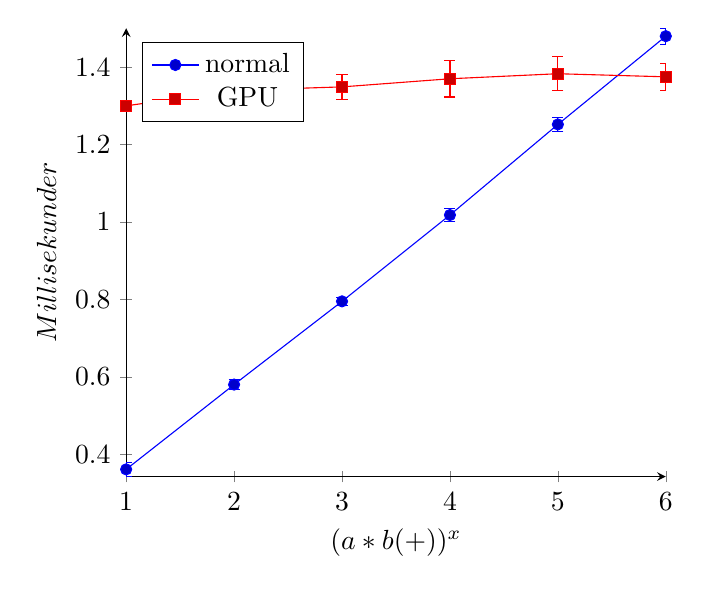
\begin{tikzpicture} 
\begin{axis}
[
    axis lines = left,
    xlabel = $ (a*b(+))^x $,
    ylabel = $Millisekunder$,
    legend pos=north west,
]

\addplot+[error bars/.cd,y dir=both,y explicit]
	coordinates 
    	{ 	
		(1,0.36100000000000004) +- (0,0.018529256146248507)
		(2,0.58000000000000007) +- (0,0.01247219128923985)
		(3,0.795) +- (0, 0.010801234497347552)
		(4,1.018) +- (0,0.016865480854228086)
		(5,1.2520000000000002) +- (0,0.018135294011630478)
		(6,1.48) +- (0,0.020548046676568125)
 }; \addlegendentry{normal}
 
 \addplot+[error bars/.cd,y dir=both,y explicit]
	coordinates 
    	{ 	
		(1,1.3) +- (0,0.01154700538377906)
		(2,1.3400000000000003) +- (0,0.039999999999992868)
		(3,1.349) +- (0, 0.032812599206197689)
		(4,1.3699999999999999) +- (0,0.047140452079106852)
		(5,1.3829999999999998) +- (0,0.043982319680124123)
		(6,1.375) +- (0,0.035355339059328042)
 }; \addlegendentry{GPU}
\end{axis} \end{tikzpicture}    
    \caption{Testen af Funcalc hvor kolonerne er fyldt ud, 1000 tal i vær kolonne, hvor \textit{A=2},\textit{B=3} og C er hvor funktioner ligger. \textit{x} står for hvor mange udredninger der er af  (a1*b1(+)) og for GPU (1*2(+)) .}
    \label{fig:Funcalc_test_2}
\end{figure}

% ------------------------------------------------------------------------------------------------------------- Funcalc test 1
\begin{figure}[p]
    \centering
   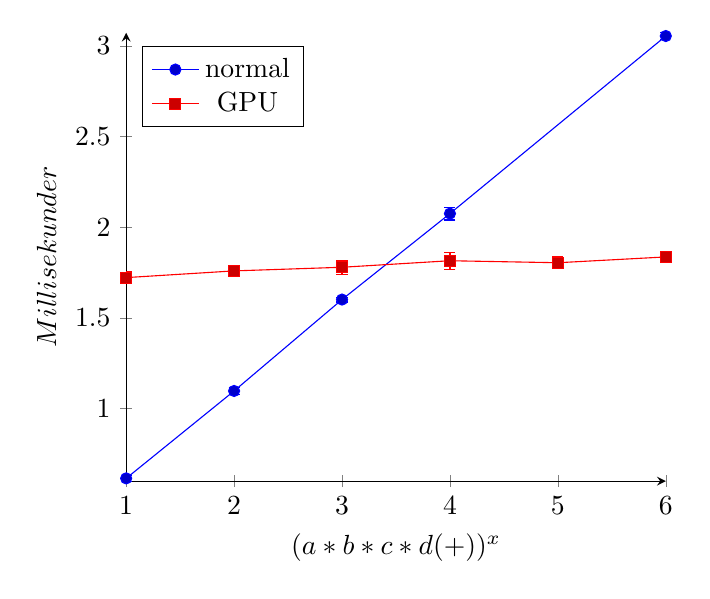
\begin{tikzpicture} 
\begin{axis}
[
    axis lines = left,
    xlabel = $ (a*b*c*d(+))^x $,
    ylabel = $Millisekunder$,
    legend pos=north west,
]

\addplot+[error bars/.cd,y dir=both,y explicit]
	coordinates 
    	{ 	
		(1,0.615) +- (0,0.015092308563562756)
		(2,1.097) +- (0,0.017669811040937646)
		(3,1.6010000000000002) +- (0, 0.013703203194048448)
		(4,2.075) +- (0.019578900207433445)
		(5,2.572) +- (0,0.035527766918592094)
		(6,3.0539999999999994) +- (0,0.017763883459407156)
 }; \addlegendentry{normal}
 \addplot+[error bars/.cd,y dir=both,y explicit]
	coordinates 
    	{ 	
		(1,1.722) +- (0,0.031198290551458049)
		(2,1.759) +- (0,0.026853512081510652)
		(3,1.779) +- (0,0.038137179293238864)
		(4,1.815) +- (0,0.0460072458061408788)
		(5,1.8040000000000003) +- (0,0.03306559138036088)
		(6,1.8359999999999999) +- (0,0.030258148581095181)
 }; \addlegendentry{GPU}
\end{axis} \end{tikzpicture}    
    \caption{Testen af Funcalc hvor kolonerne er fyldt ud, 1000 tal i vær kolonne, hvor \textit{A=B=2},\textit{C=D=3} og E er hvor funktioner ligger. \textit{x} står for hvor mange udredninger der er af  (a1*b1*c1*d1(+)) og for GPU (1*2*3*4(+)).}
    \label{fig:Funcalc_test_1}
\end{figure}



% ------------------------------------------------------------------------------------------------------------- Funcalc_test_3
\begin{figure}[p]
    \centering
   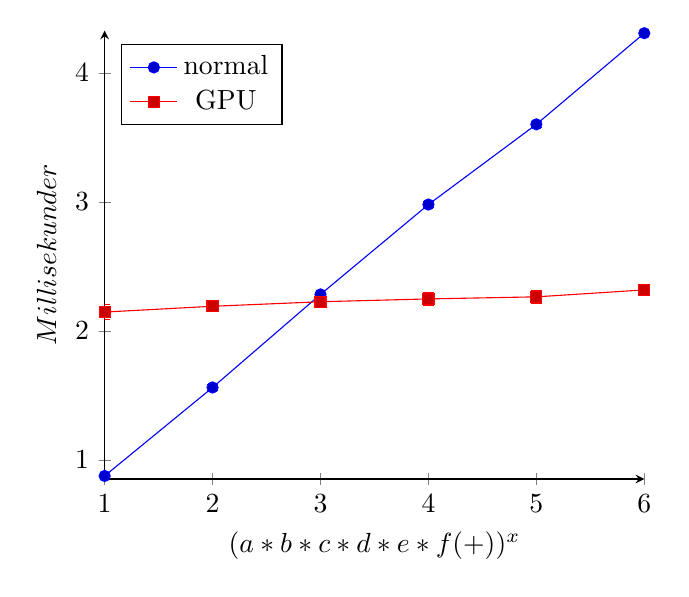
\begin{tikzpicture} 
\begin{axis}
[
    axis lines = left,
    xlabel = $ (a*b*c*d*e*f(+))^x $,
    ylabel = $Millisekunder$,
    legend pos=north west,
]

\addplot+[error bars/.cd,y dir=both,y explicit]
	coordinates 
    	{ 	
		(1,0.875) +- (0,0.023687784005917218)
		(2,1.5610000000000004) +- (0,0.024698178070420965)
		(3,2.283) +- (0,0.0141813649241456)
		(4,2.9800000000000004) +- (0,0.024944382578432223)
		(5,3.6020000000000003) +- (0,0.021499353995423059)
		(6,4.3089999999999993) +- (0,0.019692073983894557)
 }; \addlegendentry{normal}
 
 \addplot+[error bars/.cd,y dir=both,y explicit]
	coordinates 
    	{ 	
		(1,2.146) +- (0,0.057773504115462088)
		(2,2.191) +- (0,0.032472210341243694)
		(3,2.226) +- (0, 0.034058772731880335)
		(4,2.248) +- (0,0.051380930314655959)
		(5,2.2640000000000002) +- (0,0.05146735750830126)
		(6,2.3180000000000005) +- (0,0.0393841479672579)
 }; \addlegendentry{GPU}
\end{axis} \end{tikzpicture}    
    \caption{testen af Funcalc hvor kolonerne er fyldt ud, 1000 tal i vær kolonne, hvor \textit{A=B=C=2},\textit{D=E=F=3} og C er hvor funktioner ligger. \textit{x} står for hvor mange af udredningen  (a*b*c*d*e*f(+)) og for GPU (a*b*c*d*e*f(+)) .}
    \label{fig:Funcalc_test_3}
\end{figure}


% ------------------------------------------------------------------------------------------------------------- template
\begin{figure}[p]
    \centering
   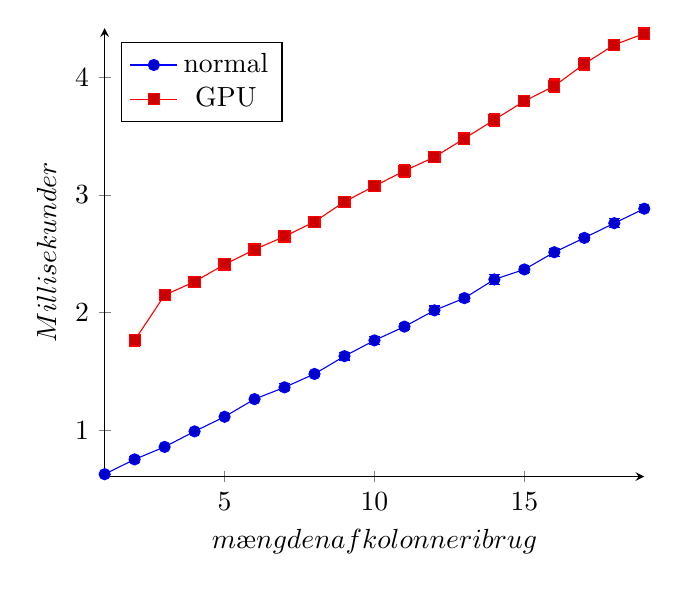
\begin{tikzpicture} 
\begin{axis}
[
    axis lines = left,
    xlabel = $mængden af kolonner i brug$,
    ylabel = $Millisekunder$,
    legend pos=north west,
]
\addplot+[error bars/.cd,y dir=both,y explicit]
	coordinates 
    	{ 	
		(1,0.628) +- (0,0.019888578520234464)
		(2,0.75400000000000011) +- (0,0.022211108331940798)
		(3,0.85999999999999976) +- (0, 0.013333333333354803)
		(4,0.992) +- (0,0.016193277068659116)
		(5,1.116) +- (0,0.01074967699772071)
		(6,1.2659999999999998) +- (0,0.015055453054211271)
		(7, 1.3659999999999999) +- (0,0.030258148581101707)
		(8,1.48) +- (0,0.021602468994685969)
		(9,1.6310000000000002) +- (0,0.03247221034121938)
		(10,1.765) +- (0,0.034721111093340619)
		(11,1.8820000000000001) +- (0,0.025733678754162138)
		(12,2.02) +- (0,0.037118429085522132)
		(13,2.1239999999999997) +- (0, 0.0279682359512392)
		(14,2.283) +- (0,0.0429599296502815)
		(15,2.368) +- (0,0.02440400695700367)
		(16,2.5140000000000002) +- (0,0.035023801430816)
		(17,2.636) +- (0,0.024585451886130674)
		(18,2.761) +- (0,0.037549966711025479)
		(19,2.8840000000000003) +- (0,0.03502380143082727)
 }; \addlegendentry{normal}
 \addplot+[error bars/.cd,y dir=both,y explicit]
	coordinates 
    	{ 	
		(2,1.7659999999999996) +- (0,0.049486249493067562)
		(3,2.149) +- (0, 0.028460498941524554)
		(4,2.264) +- (0,0.025473297566070773)
		(5,2.4100000000000006) +- (0,0.0326598632370589)
		(6,2.537) +- (0,0.031640339933539319)
		(7, 2.648) +- (0,0.029739610697615042)
		(8,2.773) +- (0,0.035605867181912138)
		(9,2.9430000000000005) +- (0,0.044484703987836334)
		(10,3.0759999999999996) +- (0,0.043256341860061255)
		(11,3.2050000000000005) +- (0,0.057203341005765553)
		(12,3.3229999999999995) +- (0,0.04056544780425788)
		(13,3.4799999999999995) +- (0, 0.040276819911983973)
		(14,3.6400000000000006) +- (0,0.052915026221245068)
		(15,3.7980000000000005) +- (0,0.043153472887122526)
		(16,3.9270000000000005) +- (0,0.059451193801629679)
		(17,4.113999999999999) +- (0,0.052957005622047214)
		(18,4.277000000000001) +- (0,0.034657049948037588)
		(19,4.372) +- (0,0.045411696975848174)
 }; \addlegendentry{GPU}
\end{axis} \end{tikzpicture}    
    \caption{Test af om mængde data der bliver arbejde på, har indflydelse på om GPU bliver bedre at arbejde på.}
    \label{fig:Test_size}
\end{figure}


\section{Diskussion}
For at først at kigge på mulighederne for at kode til en GPU til C Sharp, som er det sprog Corecalc er skrevet i, er der blevet lavet nogen forskellige test der giver nogen interessante resultater. Vis man kigger på CUDAfy og CUDA, kan man se til at CUDA kan klare små matrixers, men af alle de forskelle måder jeg har testet til at kode til en GPU, virker det til at CUDA ikke kan klare større matrixers i forhold til hvordan CUDAfy klare sig. Dette problem kunne skylle at CUDAfy måske har en smule kode optimering, mens CUDA muligvis ikke nar nogen kode optimering. grunlaget for at jeg tror dette er sandet, er at koden er stort set den sammen i for alle matrix multiplikationer.

En anden grund til at dette kunne passe er hukommelses brug af array. I CUDAfy er hukommelsen fast låst til en form for allokering af array. Hvorimod CUDA er meget åben i forhold til hvordan du vil bruge hukommelsen, i forhold til CUDAfy. Dette kunne med føre at allokering af array igennem CUDA ikke er meget optimeret, hvorimod at igennem CUDAfy er det bedre da man programøren ikke skal rode med det aspekt af kodning og er heller ikke rigtig kigge meget på, da der ikke er en god dokumentering.

en overraskende ting kan ses i CUDAfy 1d og 2d kan det ses, at det er hurtigere at, hvis håndterer data i 1d array i sted for 2d array, når matrixen begunder at blive have den størrelse være 10 eller over.
\section{Konklusion}
Formålet med dette projekt var, at prøve at gøre det det nemmere at kode til GPU igennem et regneark program.
\section{Fremtidige Arbejde}
\label{FA}
Første ting kunne være at lave lidt om på GPU funktion, så den kunne tage værdier der er den samme for alle udregninger, på dette tidspunkt kan GPU funktion kun arbejde med et \textit{array} der består af input. Men hvis GPU funktion gav lov til at sende et ekstra \textit{array} med globale værdier alle tråde skal bruge, kunne det hjælpe på overførsel tid og spare på pladsen på GPU. Dette kunne gøres ved at tillade, at når man giver lov til at markeret en celle ved bruge af GPU funktion, der sådan bliver til den global værdi, måden de globale værdier kunne pointet til i indkodning, ville være at bruge de positive tal der ikke bliver bugt for at beskrive input data. Eksempelvis kunne man skrive en GPU funktion sådan: $=GPU(A1:B10, (1+2)*C1)$. her vil den lave et \textit{array} over \textit{A1:B10} hvor hver tråd har den data i og sende et \textit{array} med \textit{C1} som alle tråde vil tilgå, for at få fadt på denne værdi.

GPU funktinon kunne blive videreudvikle, så den kan håndterer \textit{if()} og \textit{rand()}. Måden den kunne klare problemet med \textit{if()}, er ved at tilføre ekstra værdier ind ind i indkodningen. Eksempelvis kunne man se \textit{if()} som en split i en udregning, vil den nye værdi indkodning holde styr på hvilken gren man befinder sig på. Derudover skal der også lavet så funktion på GPU, som er i stand til at udregne et boolean udtryk. Udvidelsen for at læse boolean udtryk burde ikke være det store problem, men udvidelsen for at håndtere \textit{if()} er muligvis ikke liget til, siden GPU funktion skal kunne håndtere at hoppe i indkodning. \textit{CUDAFY} ser ikke ud til at have en tilfældigheds funktion i sig, så derved kan \textit{rand()} ikke gøres på GPU siden, man kunne lave nogen tilfældige tal og sende med til GPU hvis den skal et tilfældigt tal, dette ville dog sænke hurtigheden for GPU, siden at testene viser at, der helst skal være flere udregninger en mængde af data man sender, ville det ikke være hurtigere at gøre udregningerne på GPU. Dog ser det ud til at \textit{CUDA} har  en form for tilfældigheds generator med navn \textit{cuRAND}, denne funktion kunne måske blive til rådighed for \textit{CUDAfy} i fremtiden. 

Et forslag ville være at GPU funktion kan tage en \textit{funcalc} funktion, skrevet i et funktion ark, i sted for at kun kan tage et \textit{CoreCalc} udtryk. Ved at gøre dette ville bruger venligheden muligvis blive bedre. Dette burde kunne lade sig gøre, da et abstrakt syntaks træ bliver lavet i funktion arket i \textit{funcalc}.

En anden interessant ide kunne være, at give brugeren mulighed for at direkte bruge cellerne som punkt for, hvad der skal ligges sammen, GPU(a1:c5 , a1+b1+c1). Så skal GPU funktion selv finde ud af om de celler i udtrykket inden for input \textit{array} eller om det er noget udenfor der, hvilket vil gøre det til en global værdi. 

Unikke GPU funktioner kunne blive lavet over kendte algoritme problemer, en af dem kunne være det samme om der er blevet brug til at teste de forskellige sprog: matrix Multiplatikon, koden er næsten lavet til fulde, der mangler nogen små ændringer, såsom at tage matrixer, der ikke har den samme længe og højde, som input kunne denne funktion tag 2 forskellige markeret celler området.

Ideen ved dette projekt var at gøre det nemmere at kode til en GPU, dette blev aldrig testet. Derfor kunne det være interessant at lave en brugertest af GPU funktion for at se, hvad en bruger mener om funktion og om der muligvis kunne laves nogen forbedring på funktion, som ikke er kommet op under projektet arbejdes tid.

Noget andet der også kunne være interessant at teste, ville være om måden at at GPU funktion kan på sin vis \textit{compile} simpel udtryk på run time, ved brug af en indkodning og læser, ville kunne klare sig mod projekter der compiler GPU kode på run time. Dette kunne være interessant at kigge på, for at se om der er hurtigere at lave GPU kode på run time eller om der hurtigere at lave en indkodning som en GPU kan udregne efter.

\bibliographystyle{plain}
\bibliography{Bibliography/bib}
\end{document}
